\documentclass{article}
\usepackage[a4paper, total={6.5in, 10in}]{geometry}
\usepackage{float}
\usepackage{amsmath}
\usepackage{enumitem}
\usepackage{graphicx}
\usepackage{placeins} % put this in your pre-amble
\usepackage{flafter}  % put this in your pre-amble
\usepackage{spverbatim}

\title{CS-E4410 Semantic Web}
\author{
  Erdogar, Can\      \texttt{625391}
}
\date{ 2 February 2017}
\usepackage{pgfplots}
\usepackage{tikz}
\usetikzlibrary{arrows,automata}

\begin{document}

\maketitle

\section{Exploring and reading Linked Data}

\subsection{Exploring DBpedia data}

\begin{verbatim}

@prefix dbr: <http://dbpedia.org/resource/>.

dbr:Edvard_Westermarck dbo:knownFor dbr:Westermarck_effect;

						dbo:birthPlace dbr:Finland, dbr:Helsinki.
						
\end{verbatim}

\subsection{Reading DBpedia data}

\begin{verbatim}

dbr:Helsinki	owl:sameAs <http://sws.geonames.org/658225/>. 
dbr:Helsinki	owl:sameAs	<http://sws.geonames.org/658226/> . 

\end{verbatim}

\section{Presenting RDF Graphs}

\subsection{Presenting an RDF graph as triples}

\begin{verbatim}

<http://esimerkki.fi/matti>
<http://w3.org/1999/02/22/rdf-syntax-ns#type> 
<http://esimerkki.fi/Person> ;

<http://esimerkki.fi/name>
"Matti"; 

<http://esimerkki.fi/knows>
<http://esimerkki.fi/maija> ;

<http://esimerkki.fi/hasChild>
<http://esimerkki.fi/liisa>.

\end{verbatim}

$ $

$ $

$ $

$ $

$ $

$ $

$ $

$ $

$ $

$ $

\subsection{Visualizing a Turtle serialization }

It turns into rdf:type \\

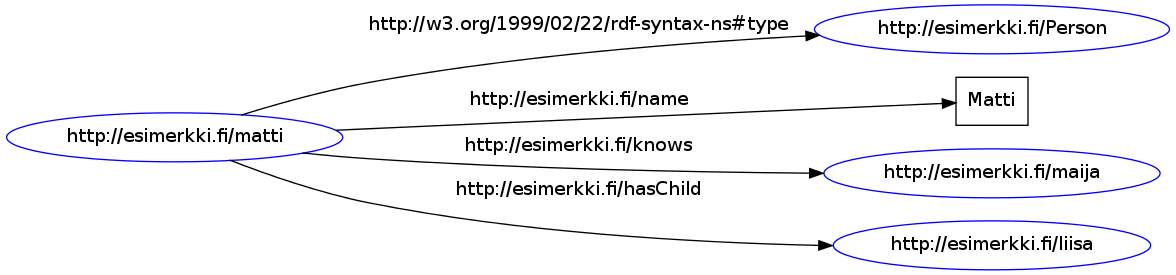
\includegraphics[width=\textwidth]{rdf-grapher.png}

\subsection{Visualizing a larger Turtle serialization}

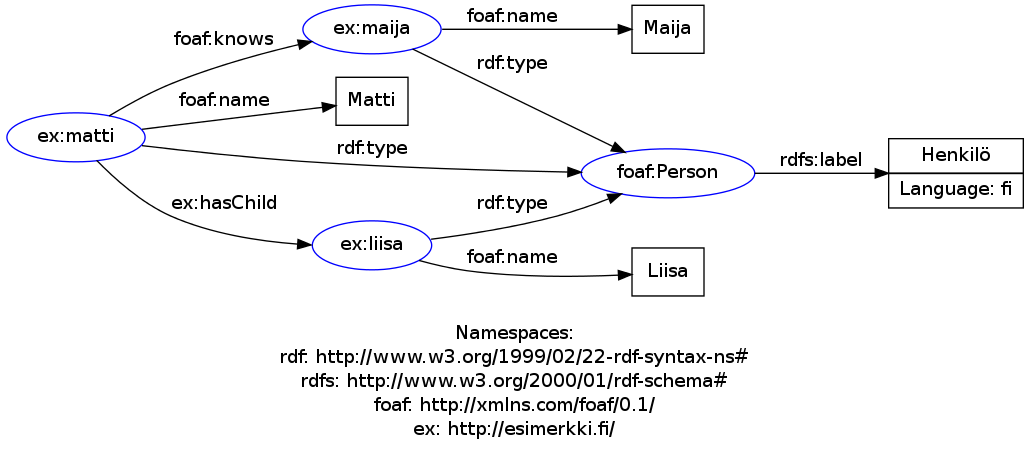
\includegraphics[width=\textwidth]{rdf-grapher2.png}

\subsection{Presenting RDF graphs in the Turtle notation}

\begin{verbatim}

@prefix ex: <http://example.com/> .
@prefix : <http://dbpedia.org/resource/>.
@prefix rdf: <http://www.w3.org/1999/02/22-rdf-syntax-ns#>.
@prefix dc: <http://purl.org/dc/elements/1.1/>.
\end{verbatim}
:r1 dc:creator "V{\"a}inö Linna"; \\
rdf:type :Romaani; \\
dc:title "T{\"a}{\"a}ll{\"a} Pohjantähden alla"@fi. \\

:r2 dc:creator "V{\"a}inö Linna"; \\
rdf:type :Romaani; \\
dc:title "Tuntematon sotilas"@fi.\\

$ $

$ $

$ $

$ $

$ $

$ $

$ $

$ $

$ $

$ $



\subsection{Converting Turtle serialization to RDF/XML}

\begin{verbatim}

<?xml version="1.0" encoding="utf-8"?>
<rdf:RDF xmlns:dc="http://purl.org/dc/elements/1.1/" xmlns:ex="http://example.com/" xmlns:rdf="http://www.w3.org/1999/02/22-rdf-syntax-ns#" 
xmlns="http://dbpedia.org /resource/" xml:base="http://www.ldf.fi/service/rdf-serializer/">
  <rdf:Description rdf:about="http://dbpedia.org/resource/r1">
    <dc:creator>Väinö Linna</dc:creator>
  </rdf:Description>
  <rdf:Description rdf:about="http://dbpedia.org/resource/r1">
    <rdf:type rdf:resource="http://dbpedia.org/resource/Romaani"/>
  </rdf:Description>
  <rdf:Description rdf:about="http://dbpedia.org/resource/r1">
    <dc:title xml:lang="fi">Täällä Pohjantähden alla</dc:title>
  </rdf:Description>
  <rdf:Description rdf:about="http://dbpedia.org/resource/r2">
    <dc:creator>Väinö Linna</dc:creator>
  </rdf:Description>
  <rdf:Description rdf:about="http://dbpedia.org/resource/r2">
    <rdf:type rdf:resource="http://dbpedia.org/resource/Romaani"/>
  </rdf:Description>
  <rdf:Description rdf:about="http://dbpedia.org/resource/r2">
    <dc:title xml:lang="fi">Tuntematon sotilas</dc:title>
  </rdf:Description>
</rdf:RDF>

\end{verbatim}

\subsection{JSON-LD notation}

$@id -->$ Used to uniquely identify things that are being described in the document with IRIs or blank node identifiers.\\

$@content -->$ Used to define the short-hand names that are used throughout a JSON-LD document. These short-hand names are called terms and help developers to express specific identifiers in a compact manner.\\

\subsection{Creating a FOAF profile}

\begin{verbatim}
@base <http://aalto.fi/>.
@prefix foaf: <http://xmlns.com/foaf/0.1/>.
@prefix dc: <http://purl.org/dc/elements/1.1/>.
@prefix xsd: <http://www.w3.org/2001/XMLSchema#>.
@prefix dbr: <http://dbpedia.org/ontology/>.

<#erdogac1> foaf:firstName "Can";
foaf:lastName "Erdogar";
foaf:birthday "1994-2-19"^^xsd:date;
foaf:topic_interest <http://www.yso.fi/onto/muso/p1114>;
dbr:birthPlace <http://sws.geonames.org/7733235/>.
\end{verbatim}

\section{RDF Schema definition}

\subsection{Defining a class hierarchy}

\begin{verbatim}
@prefix rdf: <http://w3.org/1999/02/22-rdf-syntax-ns#>.
@prefix rdfs: <http://w3.org/2000/01/rdf-schema#>.
@prefix a: <http://aalto.fi/>.

a:Work rdf:type rdfs:Class.

a:Book rdf:type rdfs:Class;
rdfs:subClassOf a:Work.

a:Composition rdf:type rdfs:Class;
rdfs:subClassOf a:Work.

a:Movie rdf:type rdfs:Class;
rdfs:subClassOf a:Work.

a:Novel rdf:type a:Book.
a:Poetry rdf:type a:Book.

a:PopMusicComposition rdf:type a:Composition.
a:ClassicalComposition rdf:type a:Composition.
\end{verbatim}

\subsection{Defining properties}

\begin{verbatim}
@prefix rdf: <http://w3.org/1999/02/22-rdf-syntax-ns#>.
@prefix rdfs: <http://w3.org/2000/01/rdf-schema#>.
@prefix a: <http://aalto.fi/>.
@prefix dc: <http://purl.org/dc/elements/1.1/>.
@prefix xmlns: <http://xmlns.com/foaf/0.1/>.
@prefix xsd: <http://www.w3.org/2001/XMLSchema#>.

a:Work rdf:type rdfs:Class.

a:Book rdf:type rdfs:Class;
rdfs:subClassOf a:Work.

a:Composition rdf:type rdfs:Class;
rdfs:subClassOf a:Work.

a:Movie rdf:type rdfs:Class;
rdfs:subClassOf a:Work.

a:Novel rdf:type a:Book.
a:Poetry rdf:type a:Book.

a:PopMusicComposition rdf:type a:Composition.
a:ClassicalComposition rdf:type a:Composition.

a:creator rdf:type rdfs:Property;
rdfs:subPropertyOf dc:creator;
rdfs:domain a:Work;
rdfs:range xmlns:Person.

a:writer rdf:type rdfs:Property;
rdfs:domain a:Book;
rdfs:range xmlns:Person.

a:composer rdf:type rdfs:Property;
rdfs:domain a:Composition;
rdfs:range xmlns:Person.

a:director rdf:type rdfs:Property;
rdfs:domain a:Movie;
rdfs:range xmlns:Person.

a:creationTime rdf:type rdfs:Property;
rdfs:domain a:Book;
rdfs:range xsd:date.

a:pageCount rdf:type rdfs:Property;
rdfs:domain a:Book;
rdfs:range xsd:integer.

\end{verbatim}

\subsection{Populating ontology with instances}

Following turtle code is the continuation of the above code.

\begin{verbatim}
a:HarryPotterandthePhilosophersStone rdf:type a:Novel;
a:writer a:JK;
a:pageCount "3"^^xsd:integer.
\end{verbatim}

\subsection{Enriching an ontology by inference}




\end{document}

​



